% main.tex
\documentclass[12pt]{article}



% Import formatting & packages
% preamble.tex
\usepackage[a4paper, margin=2.5cm]{geometry}  % Page size & margins
\usepackage{graphicx}   % Figures
\usepackage{booktabs}   % Professional tables
\usepackage{amsmath}    % Math symbols & equations
\usepackage{amssymb}    % More math symbols
\usepackage{hyperref}   % Hyperlinks
\usepackage{cleveref}   % Smart references
\usepackage{enumitem}   % Customizable lists
\usepackage{float}      % Better table/figure placement
\usepackage[utf8]{inputenc}  % Ensure Overleaf uses UTF-8 encoding
\usepackage{csquotes}   % Improved quotation formatting
\usepackage{tabularx}
\usepackage{tabularray}
\usepackage{tikz}
\usetikzlibrary{shapes.geometric, arrows}
\usepackage{pgfplotstable,siunitx,xfp}
\pgfplotsset{compat=1.18}
\usepackage{siunitx}   % \num, rounding/formatting
\usepackage{xfp}       % or expl3; xfp gives \fpeval
\usepackage{titling} 
\usepackage{verbatim} % for \verbatiminput
\newcommand*\wordcount{%
  % run texcount & save result in jobname.wc:
  \immediate\write18{texcount -merge -sum \jobname.tex > \jobname.wc}%
  % read the first line (total words) from that file
  \verbatiminput[fontsize=\small, firstline=1, lastline=1]{\jobname.wc}%
}

% Bibliography
\usepackage[backend=biber, style=authoryear, sorting=nyt]{biblatex}  
\addbibresource{references.bib}  % Link to your Zotero export

% Section number depth
\setcounter{secnumdepth}{3}

% Table & figure captions
\usepackage[labelfont=bf]{caption}  










\begin{document}

\include{titlepage}

\section{Introduction}
\textbf{500 words}

\subsection{Background}

\subsubsection{Active Learning Models for Systematic Reviewing}

Researchers and practitioners are continually challenged to base their decisions on the latest scientific evidence. Systematic reviews and meta-analyses were developed to address this need as rigorous methods of summarizing scientific literature \parencite{chalmers2002brief, bastian2010seventy}. However, systematically reviewing the literature can be time-consuming, which limits its practical applicability, especially, in, for example, times of crisis \parencite{tricco2020rapid, nussbaumer2021resource}.

Fortunately, recent advances in machine learning have produced tools that allow for the systematic screening of scientific literature while greatly reducing the need for manual screening \parencite{van2021open}. Specifically, active learning models (ALMs) ask users to screen titles and abstracts of papers one by one. Based on the user's decision, the models reassess the probability that the remaining papers are relevant and thus whether to show them to the user. In other words, these models continually reshuffle the papers retrieved from a scientific literature search based on the user's interests. This method reduces the time needed to find as many relevant papers as possible compared to simple index-based screening \parencite{van2025hunt}. 

\subsubsection{The Cold Start Problem}

A key challenge to using active learning for systematic reviews is that these models face a "cold start" \parencite{panda2022approaches}. For an ALM to query a user with a potentially interesting paper, the model must first have knowledge of the user's interests . One way of overcoming a cold start is to initialize, or 'warm up', the ALM using examples of relevant and irrelevant papers \parencite{teijema2025large}. If however no examples are available the user may simply start screening papers at random, until a relevant and an irrelevant paper have been found. 

\subsubsection{The Advent of Large Language Models}

With the recent advent of large language models (LLMs), a new possible solution to overcoming the cold start problem has emerged \parencite{bachmann2025adaptive}. Instead of screening papers at random until relevant and irrelevant examples are found, LLMs can generate synthetic examples of both based on the systematic review's inclusion and exclusion criteria. This approach may be particularly advantageous when the percentage of relevant papers returned by a systematic search is low. In this case, screening using even suboptimal examples of relevant and irrelevant papers may be preferable to randomly screening hundreds or thousands of papers. In other words, something may be better than nothing. However, synthetic data may also misdirect the ALM by contaminating the model's training data. 

In summary, the 'cold start' problem may be overcome and the performance of ALM-assisted screening improved by initialising the ALM with relevant and irrelevant paper examples generated by LLMs. This approach could be particularly useful if a user has no relevant examples available, as it avoids random screening. A key question, however, is whether LLM-generated examples improve starting performance beyond that achieved through initialisation using the systematic review's inclusion and exclusion criteria directly.


\subsection{Objectives}

This study aims to investigate the effect of using LLM-generated data to initialise active learning models (ALMs) for systematic reviews, compared to random initialisation, no initialisation or criteria-based initialisation, on starting performance. This will be achieved by simulating the screening of previously published systematic reviews.

% The aim is to investigate the effect \textit{on starting performance} of initializing  ALMs for systematic reviews using:
% \begin{enumerate}[label=\arabic*), leftmargin=*, nosep]
%     \item examples of relevant and irrelevant papers generated by LLMs;
%     \item examples of relevant and irrelevant papers randomly sampled from the sets of screened papers;
%     \item without any examples,
% \end{enumerate}

\section{Methodology}
\textbf{1000 words}

\subsection{Conditions}

This study aims to compare the effect of LLM initialisation with that of three control conditions: random initialisation, no initialisation, and criteria-based initialisation. In all conditions except the 'no initialisation' condition, the LLM is initialised using only relevant papers. This is because systematic reviews contain a large number of irrelevant papers, meaning they no 'cold start' problem.

\subsubsection{Experimental condition: LLM initialization}

In the LLM initialisation condition, the ALM's classifier is provided with a set of examples comprising at least one relevant paper before screening is simulated. These examples are generated based on the inclusion and exclusion criteria of the given systematic review publication. See figure \ref{fig:sim-pipeline} for a schematic of the simulation pipeline. 

Between simulation runs the exact number of abstracts generated as well as their specific contents is varied. More specifically, we aimed to investigate the effect of the following variables on starting performance: 
\begin{enumerate}[label=\arabic*)]
\item number of abstracts generated per simulation run \textit{(1, 4 or 7 abstracts)},
\item length of abstracts generated per simulation run \textit{(200, 500, 1000 words)},
\item the temperature setting on the LLM \textit{(0.0, 0.4, 0.8)},
\end{enumerate}

To instruct the LLM, a DSPY module was created which takes the variables described above as input, along with the inclusion and exclusion criteria of the systematic review and a generic prompt \parencite{khattab2023dspy}. The module then generates the desired number of abstracts using OpenAI's gpt-4o-mini model. For the exact code, see: \href{https://github.com/timovanommeren/thesis_timo/blob/main/simulations/prompting.py}{here}

\subsubsection{Control conditions}

In the \textit{random initialization} condition, one relevant paper was sampled at random prior to the start of screening (with replacement between runs). In the \textit{criteria-based initialisation}, the inclusion and exclusion criteria of the systematic review directly functioned as an example of an abstract of a relevant paper with which to initialise the ALM. In the \textit{no initialisation} condition, no papers were provided prior to the start of screening.


\subsection{Outcome variable}

\subsubsection{Starting performance}

Starting performance will be assessed based on the number relevant papers in the first 100 papers screened. This figure is derived from research showing that approximately 100 papers can be screened in an hour \parencite{nussbaumer2021resource}. For each simulation, we count the number of relevant records found with a \textit{Time to Discovery} below 100 for each simulation \parencite{ferdinands2023performance}.

\subsection{Simulation set-up}

In order to investigate the effect between LLM initialisation and the control conditions on starting performance, the SYNERGY datasets will be screened based on the abstracts and titles of the papers using ASReview's ALM \parencite{van2021open, de2023synergy}. 

ASReview is an open-source software package for semi-automated systematic reviewing that implements several ALMs. To simulate the screening process, we will access ASReview via its Python API. For all simulation runs, we will set the ALM to the recommended U4 configuration in ASReview, which combines a support vector machine classifier (seeded with the run number) with a bi-gram term-frequency inverse document frequency (TF-IDF) feature extractor and a querier which always present the next most likely paper \footnote{Note that two ALMs are technically used. A simple random querier is initially used to find at least one relevant and one irrelevant paper, including initialisation examples. After this, the U4 is used.}. 

The SYNERGY datasets consist of 24 previously screened and labelled sets of papers. Importantly, this gives us access to the ground truth labels of all the papers in these datasets. See Appendix \ref{tab:SYNERGY} for a list of all datasets including their topic, total number of records, number of records included and the percentage of relevant records \parencite{de2023synergy}. 

All simulations were done in \textit{Python version 3.10}. For all the code aswell as the full list of the packages and their versions, please see \href{https://github.com/timovanommeren/thesis_timo}{the github repository}. See appendix \ref{sec:format_exported_simulation_results} for a detailed description of how the simulation results were exported.


\hspace{1cm}

\begin{figure}[htbp]
  \centering
    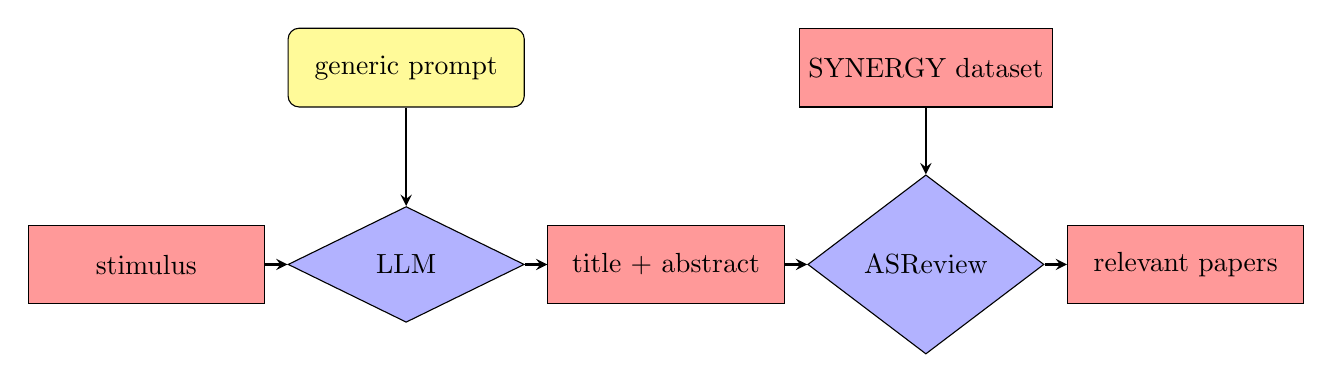
\begin{tikzpicture}[node distance=2.5cm]
    
    \tikzstyle{data} = [rectangle, minimum width=3cm, minimum height=1cm,text centered, draw=black, fill=red!40]
    \tikzstyle{prompt} = [rectangle, rounded corners, minimum width=3cm, minimum height=1cm,text centered, draw=black, fill=yellow!40]
    \tikzstyle{process} = [diamond, minimum width=3cm, minimum height=1cm, text centered, draw=black, fill=blue!30]
    \tikzstyle{arrow} = [thick,->,>=stealth]
    
    % \tikzstyle{io} = [trapezium, trapezium left angle=70, trapezium right angle=110, minimum width=3cm, minimum height=1cm, text centered, draw=black, fill=blue!30]
    % \tikzstyle{process} = [rectangle, minimum width=3cm, minimum height=1cm, text centered, draw=black, fill=red!30]
    
    \node[data]    (stim) {stimulus};
    \node[process, right of=stim, xshift=0.8cm] (llm) {LLM};
    \node[prompt,    above of=llm]  (prom)  {generic prompt};
    \node[data,    right of=llm, xshift=0.8cm]  (ta)  {title + abstract};
    \node[process, right of=ta, xshift=0.8cm]   (asr) {ASReview};
    \node[data,    above of=asr]  (syn)  {SYNERGY dataset};
    \node[data,    right of=asr, xshift=0.8cm]  (rel) {relevant papers};
    
    \draw[arrow] (stim) -- (llm);
    \draw[arrow] (prom) -- (llm);
    \draw[arrow] (llm)  -- (ta);
    \draw[arrow] (ta)   -- (asr);
    \draw[arrow] (syn)   -- (asr);
    \draw[arrow] (asr)  -- (rel);
    
    \end{tikzpicture}
    \caption{Simulation pipeline (for more detailed schematic of workings within ASReview see \parencite{asreviewvs2jonathan})}
  \label{fig:sim-pipeline}
\end{figure}

\subsection{Data Generation and Analysis}

\subsubsection{Padding}

It is important to note that the simulation may stop prematurely if all the relevant records are found before the stopping rule is reached (e.g. after screening 100 records). To accurately emulate a researcher who is unaware that all the relevant records have been found and therefore continues screening until the stopping rule is reached, the simulation results were supplemented with rows containing the label 'zero' (i.e. irrelevant records) until the stopping rule would have been reached. This process is referred to as 'padding' and ensures that the final simulation results are accurate.

\subsubsection{Analysis}

The majority of the variance in the number of relevant records found in the first 100 screened is expected to be explained by differences between datasets. We would therefore like to seperate within-dataset variance from between-dataset variance. Ideal for this purpose are multilevel regression models which allow us to model the effect of condition on starting performance while accounting for between-dataset variance by including dataset as a random effect. To confirm that most of the variance is indeed between datasets, we will visualize the data using boxplots and fit a null model with only dataset as a random effect to calculate the intraclass correlation coefficient (ICC). An exploratory bottom-up modelling approach will then be used for multilevel analysis (for approach see chapter 4 of the book by \cite{hox2017multilevel}) and will be conducted in R using the \textit{lme4} package \parencite{bates2015fitting}. %(version 1.1.36)

Note that in the control conditions, the independent variables (i.e., number of abstracts, length of abstracts, temperature) are not applicable, and will therefore be coded as missing. To account for this apparent missingness, a dummy variable indicating whether the condition is the LLM initialisation condition or not will be included in the model using the approach described by \parencite{dziak2017two}

\section{Results (note: preliminary!)}

\subsection{Descriptives}

As expected, most of the variance in starting performance seems to be explained by differences between datasets. Figure \ref{fig:all-datasets} shows the number of relevant records found within the first 100 screened per dataset. This may be partly explained by the considerable variation in the number of relevant records present in each dataset. In fact, all relevant records were found in within the first 100 screened records, in , 6.91\% of the runs in the LLM-initialization condition. In the random-initialization condition, this was 0\%, in the criteria condition, 8.08\%, and in the no-initialization condition, 1.52\%.



\begin{figure}[htbp]
  \centering
  \includegraphics[width=1\textwidth]{results/td_barchart.png} % adjust path/width
  \caption{The number of relevant records found per dataset}
  \label{fig:all-datasets}
\end{figure}

\subsection{Main results}

\input{results/results_paragraph.tex}

\begin{figure}[htbp]
  \centering
  \includegraphics[width=0.45\textwidth]{aggregate_recall_plot_walker.png}
  \includegraphics[width=0.45\textwidth]{aggregate_recall_plot_moran.png}
  \caption{The number of relevant records found per dataset}
  \label{fig:walker-2018}
\end{figure}



% Table created by stargazer v.5.2.3 by Marek Hlavac, Social Policy Institute. E-mail: marek.hlavac at gmail.com
% Date and time: Wed, Nov 19, 2025 - 21:35:44
\begin{table}[!htbp] \centering 
  \caption{Effect of initialisation on the number relevant records found in first 100 screened} 
  \label{} 
\begin{tabular}{@{\extracolsep{5pt}}lccccc} 
\\[-1.8ex]\hline 
\hline \\[-1.8ex] 
 & \multicolumn{5}{c}{\textit{Dependent variable:}} \\ 
\cline{2-6} 
\\[-1.8ex] & \multicolumn{5}{c}{Outcome: number of records found} \\ 
\\[-1.8ex] & (1) & (2) & (3) & (4) & (5)\\ 
\hline \\[-1.8ex] 
 \multirow{2}{*}{\shortstack[l]{Random\\initialisation}} & $-$0.766 & $-$0.766 & $-$0.766 & $-$0.766 & $-$0.766 \\ 
  & (0.377) & (0.377) & (0.377) & (0.768) & (0.742) \\ 
  & & & & & \\ 
 \multirow{2}{*}{\shortstack[l]{No\\initialisation}} & $-$14.420 & $-$14.420 & $-$14.420 & $-$14.420 & $-$14.420 \\ 
  & (0.377) & (0.377) & (0.377) & (4.123) & (3.929) \\ 
  & & & & & \\ 
 \multirow{2}{*}{\shortstack[l]{Number of \\ abstracts}} &  & 0.079 & 0.079 & 0.079 & 0.079 \\ 
  &  & (0.188) & (0.188) & (0.040) & (0.040) \\ 
  & & & & & \\ 
 \multirow{2}{*}{\shortstack[l]{Length \\ abstracts}} &  & $-$0.00004 & $-$0.00004 & $-$0.00004 & $-$0.00004 \\ 
  &  & (0.0005) & (0.0005) & (0.0001) & (0.0001) \\ 
  & & & & & \\ 
 \multirow{2}{*}{\shortstack[l]{LLM \\ temperature.}} &  & 0.121 & 0.121 & 0.121 & 0.121 \\ 
  &  & (0.451) & (0.451) & (0.097) & (0.097) \\ 
  & & & & & \\ 
 \multirow{2}{*}{\shortstack[l]{Dataset size \\ (N records)}} &  &  & 6.400 & 1.927 & 1.927 \\ 
  &  &  & (2.570) & (2.326) & (2.326) \\ 
  & & & & & \\ 
 \multirow{2}{*}{\shortstack[l]{\% relevant records}} &  &  & 2.294 & 2.413 & 1.616 \\ 
  &  &  & (0.468) & (0.423) & (0.651) \\ 
  & & & & & \\ 
 \multirow{2}{*}{\shortstack[l]{\% x Random \\ initialisation}} &  &  &  &  & 0.184 \\ 
  &  &  &  &  & (0.135) \\ 
  & & & & & \\ 
 \multirow{2}{*}{\shortstack[l]{\% x No initialisation}} &  &  &  &  & 1.159 \\ 
  &  &  &  &  & (0.716) \\ 
  & & & & & \\ 
 Constant & 30.882 & 30.882 & 30.882 & 30.882 & 30.882 \\ 
  & (3.471) & (3.471) & (2.475) & (3.615) & (3.512) \\ 
  & & & & & \\ 
\hline \\[-1.8ex] 
$\mathrm{Var}(u_{0j})$ & 311.447 & 311.447 & 157.375 & 339.764 & 320.599 \\ 
$\mathrm{Var}(u_{1j})$ &  &  &  & 15.158 & 14.133 \\ 
$\mathrm{Var}(u_{2j})$ &  &  &  & 441.751 & 401.266 \\ 
$\mathrm{Var}(\varepsilon_{ij})$ & 99.757 & 99.751 & 99.751 & 4.596 & 4.596 \\ 
$\rho(u_{0j}, u_{1j})$ &  &  &  & -0.297 & -0.251 \\ 
$\rho(u_{0j}, u_{2j})$ &  &  &  & -0.787 & -0.772 \\ 
$\rho(u_{1j}, u_{2j})$ &  &  &  & 0.383 & 0.331 \\ 
$\Delta$ deviance (df) &  & 0.25 (3) & 17.7 (2)*** & 12563.22 (5)*** & 3.19 (2) \\ 
Log Likelihood & $-$15,750.910 & $-$15,750.780 & $-$15,741.930 & $-$9,460.322 & $-$9,458.725 \\ 
Akaike Inf. Crit. & 31,511.820 & 31,517.560 & 31,503.870 & 18,950.640 & 18,951.450 \\ 
\hline 
\hline \\[-1.8ex] 
\multicolumn{6}{l}{Model 1: only initialization conditions.} \\ 
\multicolumn{6}{l}{Model 2: adds within-dataset covariates.} \\ 
\multicolumn{6}{l}{Model 3: adds between-dataset covariates.} \\ 
\multicolumn{6}{l}{Model 4: adds random effects for initialization.} \\ 
\multicolumn{6}{l}{Model 5: adds interaction terms.} \\ 
\multicolumn{6}{l}{$^{*} p<0.1; ^{**} p<0.05; ^{***} p<0.01$} \\ 
\end{tabular} 
\end{table} 


\section{Conclusion} 

The results of this simulation study provide a proof of concept that LLM-initialization can improve starting performance of active learning models for systematic reviews compared no initialisation. Exploratory analyses suggest that the exact instructions given to the LLM (i.e., prompt engineering) does not seem to have a large effect on starting performance. The key lesson is thus that when it comes to active learning models for systematic reviews, something is better than nothing when it comes to initialisation. We thus recommend that researchers and practitioners consider using LLM-generated examples of relevant and irrelevant papers to initialise active learning models for systematic reviews, especially when no actual examples are available. However, future work should investigate whether initialisation using LLM-generated examples does not negatively impact the overall performance or last-to-find performance of active learning models for systematic reviews by contaminating the training data of these models. Moreover, future work should investigate whether these results generalize to real-world systematic reviews, as the current simulation study may have been affected by data leakage (i.e., LLMs have been trained on synergy datasets).





\section{Discussion}



\begin{figure}[htbp]
  \centering
  \includegraphics[width=0.2\textwidth]{vector_space/LLM_vector_space.png}
  \includegraphics[width=0.2\textwidth]{vector_space/random_vector_space.png}
  \includegraphics[width=0.2\textwidth]{vector_space/no_vector_space.png}
  \caption{Ideal starting point for systematic reviews using active learning}
  \label{fig:my-image}
\end{figure}

In other words, whether, in the case of AI-assisted reviewing, prompt engineering actually aids in knowledge discovery or whether LLMs simply repackage existing knowledge.

More LLM-specific variables were considered in advance (such as degree of jargon), however, because early simulations showed difference between the LLM- and criteria-based initialisation conditions, these variables were not further investigated. Future work may consider these variables in more detail.

Since many datasets have less than a 100 relevant records, operationalizing starting performance as the number of relevant records found in the first 100 screened may be limiting, as in some runs all relevant records are found before the stopping rule is reached (). How quickly all relevant records are found is now not considered. Future work may consider alternative operationalizations of starting performance which take this into account.

Most eligibility criteria are written in either conjunctive or disjunctive form. In the latter case, all the inclusion criteria must be met for a paper to be included, whereas in the former, only one must be met. This may affect how useful LLM-generated examples are compared to using the eligibility criteria directly or selecting random examples. This is because, for criteria in conjunctive form, abstracts will be relevant if and only if all the terms from the eligibility criteria are mentioned. In contrast, for criteria in in disjunctive form, the relevant abstracts will likely only contain one of the many terms mentioned in the eligibility criteria. 

\subsection{Limitations}

\begin{enumerate}
    \item Key limitation simulation study: data leakage (i.e., LLMs have been trained on synergy datasets). The ecological validity of the results are therefore somewhat limited.
    \begin{enumerate}
        \item There are two obvious solutions to the problem of data leakage: (1) apply the use of LLm-initialization on a new systematic review, and (2) use an older LLM from hugging face for example. 
    \end{enumerate}
    \item Another possible limitation: no switching of active leaning cycles (could fix contamination of synthetic data issue). 
\end{enumerate}

Clusters should not be a problem because we only focus on starting performance (i.e., first 100 screened). Future work may consider the contamination hypothesis in more detail. 

%TC:ignore

\appendix

\section{SYNERGY metadata}

\begin{table}[ht]
\centering
\caption{Datasets overview}
\begin{tabularx}{\textwidth}{@{}r l X r r r@{}}
\toprule
\textbf{Nr} & \textbf{Dataset} & \textbf{Topic(s)} & \textbf{Records} & \textbf{Included} & \textbf{\%} \\
\midrule
1  & Appenzeller-Herzog\_2019 & Medicine & 2873  & 26  & 0.9 \\
2  & Bos\_2018                 & Medicine & 4878  & 10  & 0.2 \\
3  & Brouwer\_2019             & Psychology, Medicine & 38114 & 62  & 0.2 \\
4  & Chou\_2003                & Medicine & 1908  & 15  & 0.8 \\
5  & Donners\_2021             & Medicine & 258   & 15  & 5.8 \\
6  & Hall\_2012                & Computer science & 8793  & 104 & 1.2 \\
7  & Leenaars\_2019            & Psychology, Chemistry, Medicine & 5812  & 17  & 0.3 \\
8  & Leenaars\_2020            & Medicine & 7216  & 583 & 8.1 \\
9  & Meijboom\_2021            & Medicine & 882   & 37  & 4.2 \\
10 & Menon\_2022               & Medicine & 975   & 74  & 7.6 \\
11 & Moran\_2021               & Biology, Medicine & 5214  & 111 & 2.1 \\
12 & Muthu\_2021               & Medicine & 2719  & 336 & 12.4 \\
13 & Nelson\_2002              & Medicine & 366   & 80  & 21.9 \\
14 & Oud\_2018                 & Psychology, Medicine & 952   & 20  & 2.1 \\
15 & Radjenovic\_2013          & Computer science & 5935  & 48  & 0.8 \\
16 & Sep\_2021                 & Psychology & 271   & 40  & 14.8 \\
17 & Smid\_2020                & Computer science, Mathematics & 2627  & 27  & 1.0 \\
18 & van\_de\_Schoot\_2018     & Psychology, Medicine & 4544  & 38  & 0.8 \\
19 & van\_der\_Valk\_2021      & Medicine, Psychology & 725   & 89  & 12.3 \\
20 & van\_der\_Waal\_2022      & Medicine & 1970  & 33  & 1.7 \\
21 & van\_Dis\_2020            & Psychology, Medicine & 9128  & 72  & 0.8 \\
22 & Walker\_2018              & Biology, Medicine & 48375 & 762 & 1.6 \\
23 & Wassenaar\_2017           & Medicine, Biology, Chemistry & 7668  & 111 & 1.4 \\
24 & Wolters\_2018             & Medicine & 4280  & 19  & 0.4 \\
\bottomrule
\end{tabularx}
\caption{Please note that two of the datasets included in the original SYNERGY dataset were excluded entirely due to data quality issues: Chou (2003) and Jeyaraman (2020). For one dataset (Moran, 2021), an updated version was used due to data quality issues in the original version.}
\end{table}
\label{tab:SYNERGY}

\section{Format exported simulation results} \label{sec:format_exported_simulation_results}

Each simulation run is stored in a separate CSV file. Every row represents a screened paper and contains the following information:

\begin{enumerate}[label=\arabic*), leftmargin=*, nosep]
  \item The paper's record ID,
  \item The assigned label (i.e., relevant or irrelevant),
  \item The classifier, querier, balancer and feature extractor used,
  \item The size of the training set,
  \item A time tag.
\end{enumerate} 

Furthermore, the following naming convention is used for the CSV files: \newline condition\_run\_run\_IVs\_n\_abstracts\_length\_abstracts\_llm\_temperature.csv. The same naming convention is used for the recall plots of each simulation run and for the generated abstracts in the LLM initialisation condition.

Finally, at the end of each run, the current values of the input parameters, the outcome variables and other relevant metadata are appended to a long format master dataframe for analysis. The columns of this dataframe are as follows:

\begin{enumerate}[label=\arabic*), leftmargin=*, nosep]
    \item the name of the outcome variable
    \item the value of the outcome variable
    \item name of the simulated dataset,
    \item the condition,
    \item the values of the independent variables (NaN for the control conditions):
        \begin{enumerate}
        \item number of abstracts
        \item length of the abstracts
        \item temperature settings of the llm (i.e., diversity)
        \end{enumerate}
    \item timestamp
    \item the run number
\end{enumerate}

This yields a data-frame containing one observation for each combination of dataset (n=26), condition (n=3), independent variables and their levels (n=$3 \times 4 \times 4 \times 5 \times 5 = 1200$), and run (n=1), thus with $26 \times 3 \times 1200 \times 1 = 93600$ rows, and the 12 columns enumerated above. 

% References
\printbibliography
%TC:endignore

\end{document}
